\documentclass[1p]{elsarticle_modified}
%\bibliographystyle{elsarticle-num}

%\usepackage[colorlinks]{hyperref}
%\usepackage{abbrmath_seonhwa} %\Abb, \Ascr, \Acal ,\Abf, \Afrak
\usepackage{amsfonts}
\usepackage{amssymb}
\usepackage{amsmath}
\usepackage{amsthm}
\usepackage{scalefnt}
\usepackage{amsbsy}
\usepackage{kotex}
\usepackage{caption}
\usepackage{subfig}
\usepackage{color}
\usepackage{graphicx}
\usepackage{xcolor} %% white, black, red, green, blue, cyan, magenta, yellow
\usepackage{float}
\usepackage{setspace}
\usepackage{hyperref}

\usepackage{tikz}
\usetikzlibrary{arrows}

\usepackage{multirow}
\usepackage{array} % fixed length table
\usepackage{hhline}

%%%%%%%%%%%%%%%%%%%%%
\makeatletter
\renewcommand*\env@matrix[1][\arraystretch]{%
	\edef\arraystretch{#1}%
	\hskip -\arraycolsep
	\let\@ifnextchar\new@ifnextchar
	\array{*\c@MaxMatrixCols c}}
\makeatother %https://tex.stackexchange.com/questions/14071/how-can-i-increase-the-line-spacing-in-a-matrix
%%%%%%%%%%%%%%%

\usepackage[normalem]{ulem}

\newcommand{\msout}[1]{\ifmmode\text{\sout{\ensuremath{#1}}}\else\sout{#1}\fi}
%SOURCE: \msout is \stkout macro in https://tex.stackexchange.com/questions/20609/strikeout-in-math-mode

\newcommand{\cancel}[1]{
	\ifmmode
	{\color{red}\msout{#1}}
	\else
	{\color{red}\sout{#1}}
	\fi
}

\newcommand{\add}[1]{
	{\color{blue}\uwave{#1}}
}

\newcommand{\replace}[2]{
	\ifmmode
	{\color{red}\msout{#1}}{\color{blue}\uwave{#2}}
	\else
	{\color{red}\sout{#1}}{\color{blue}\uwave{#2}}
	\fi
}

\newcommand{\Sol}{\mathcal{S}} %segment
\newcommand{\D}{D} %diagram
\newcommand{\A}{\mathcal{A}} %arc


%%%%%%%%%%%%%%%%%%%%%%%%%%%%%5 test

\def\sl{\operatorname{\textup{SL}}(2,\Cbb)}
\def\psl{\operatorname{\textup{PSL}}(2,\Cbb)}
\def\quan{\mkern 1mu \triangleright \mkern 1mu}

\theoremstyle{definition}
\newtheorem{thm}{Theorem}[section]
\newtheorem{prop}[thm]{Proposition}
\newtheorem{lem}[thm]{Lemma}
\newtheorem{ques}[thm]{Question}
\newtheorem{cor}[thm]{Corollary}
\newtheorem{defn}[thm]{Definition}
\newtheorem{exam}[thm]{Example}
\newtheorem{rmk}[thm]{Remark}
\newtheorem{alg}[thm]{Algorithm}

\newcommand{\I}{\sqrt{-1}}
\begin{document}

%\begin{frontmatter}
%
%\title{Boundary parabolic representations of knots up to 8 crossings}
%
%%% Group authors per affiliation:
%\author{Yunhi Cho} 
%\address{Department of Mathematics, University of Seoul, Seoul, Korea}
%\ead{yhcho@uos.ac.kr}
%
%
%\author{Seonhwa Kim} %\fnref{s_kim}}
%\address{Center for Geometry and Physics, Institute for Basic Science, Pohang, 37673, Korea}
%\ead{ryeona17@ibs.re.kr}
%
%\author{Hyuk Kim}
%\address{Department of Mathematical Sciences, Seoul National University, Seoul 08826, Korea}
%\ead{hyukkim@snu.ac.kr}
%
%\author{Seokbeom Yoon}
%\address{Department of Mathematical Sciences, Seoul National University, Seoul, 08826,  Korea}
%\ead{sbyoon15@snu.ac.kr}
%
%\begin{abstract}
%We find all boundary parabolic representation of knots up to 8 crossings.
%
%\end{abstract}
%\begin{keyword}
%    \MSC[2010] 57M25 
%\end{keyword}
%
%\end{frontmatter}

%\linenumbers
%\tableofcontents
%
\newcommand\colored[1]{\textcolor{white}{\rule[-0.35ex]{0.8em}{1.4ex}}\kern-0.8em\color{red} #1}%
%\newcommand\colored[1]{\textcolor{white}{ #1}\kern-2.17ex	\textcolor{white}{ #1}\kern-1.81ex	\textcolor{white}{ #1}\kern-2.15ex\color{red}#1	}

{\Large $\underline{12n_{0524}~(K12n_{0524})}$}

\setlength{\tabcolsep}{10pt}
\renewcommand{\arraystretch}{1.6}
\vspace{1cm}\begin{tabular}{m{100pt}>{\centering\arraybackslash}m{274pt}}
\multirow{5}{120pt}{
	\centering
	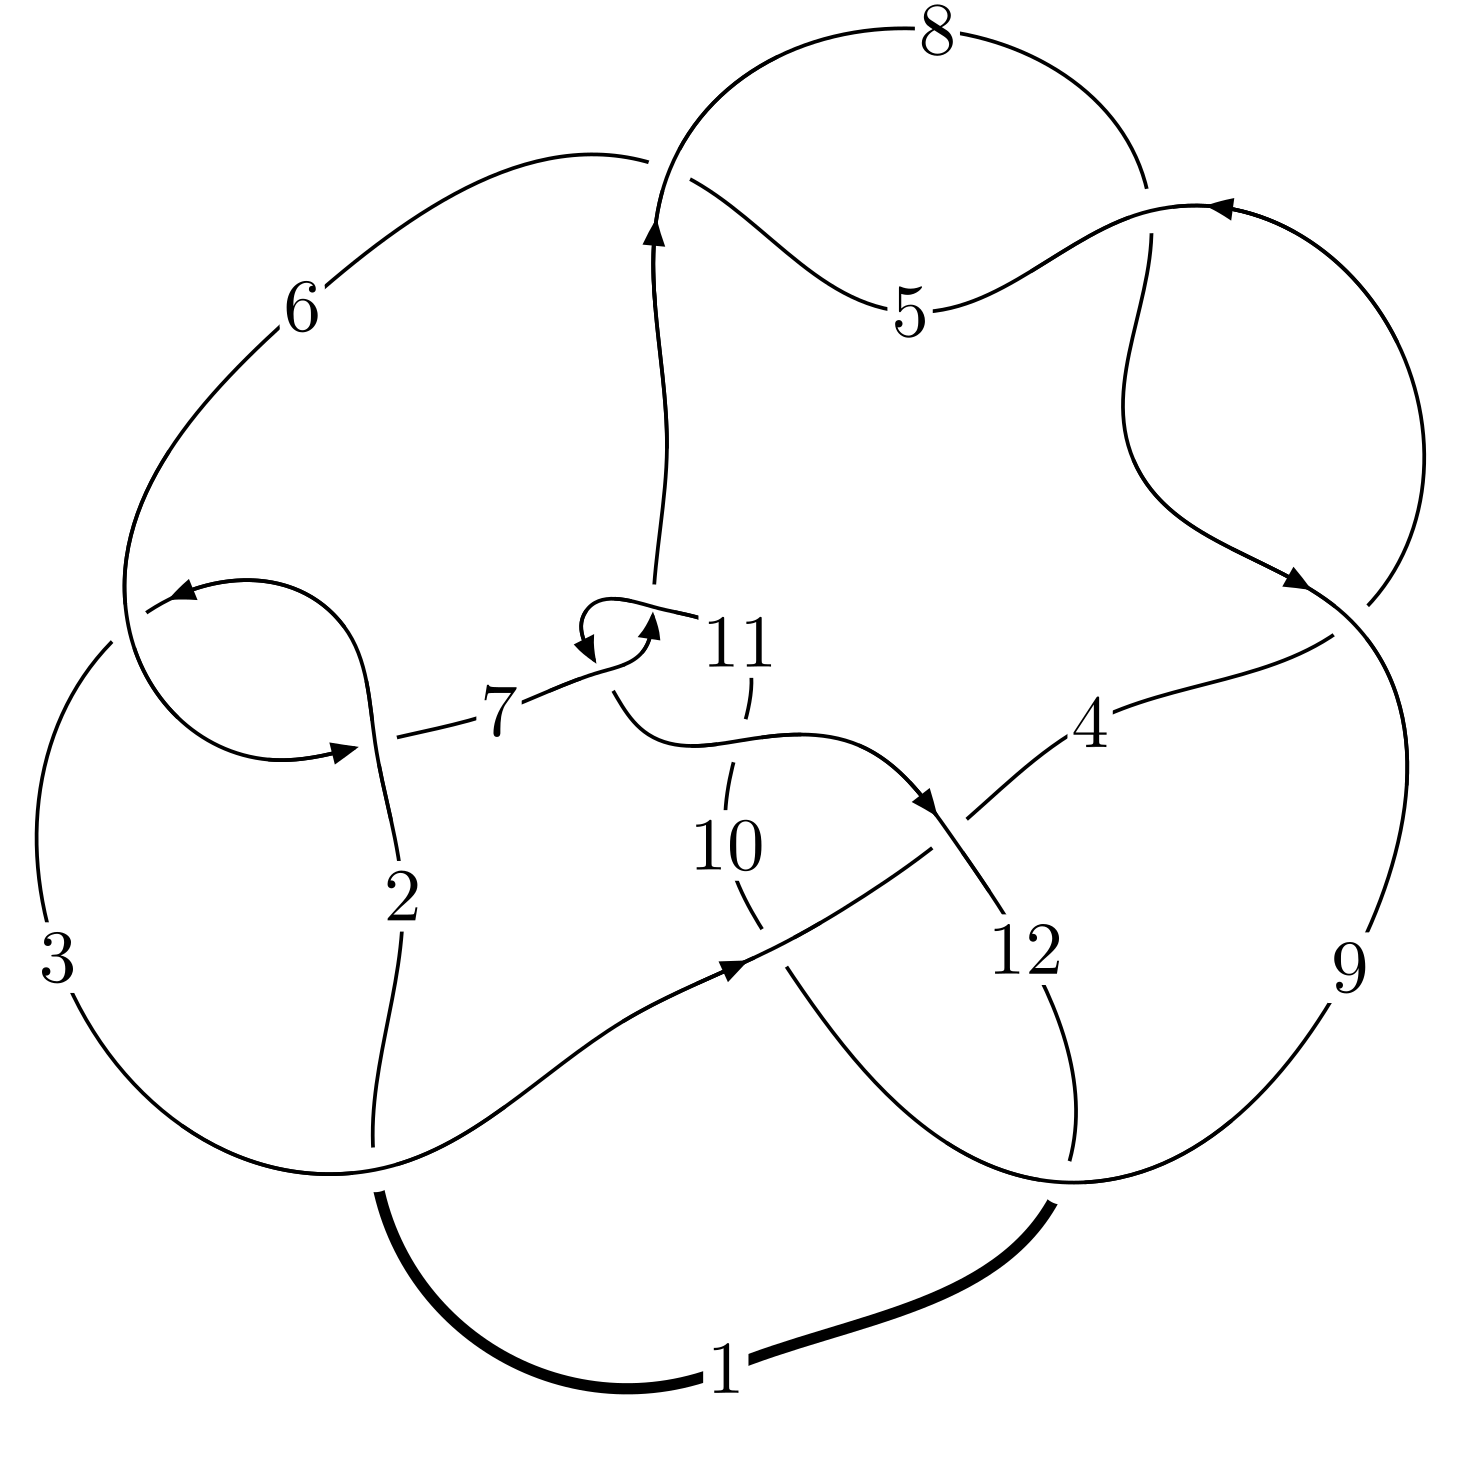
\includegraphics[width=112pt]{../../../GIT/diagram.site/Diagrams/png/2613_12n_0524.png}\\
\ \ \ A knot diagram\footnotemark}&
\allowdisplaybreaks
\textbf{Linearized knot diagam} \\
\cline{2-2}
 &
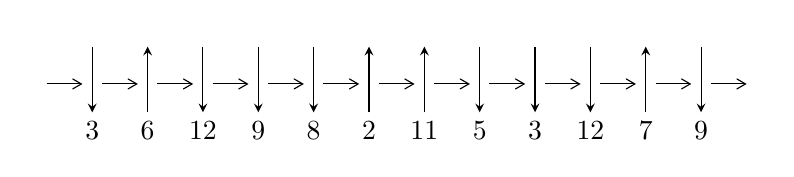
\begin{tikzpicture}[x=20pt, y=17pt]
	% nodes
	\node (C0) at (0, 0) {};
	\node (C1) at (1, 0) {};
	\node (C1U) at (1, +1) {};
	\node (C1D) at (1, -1) {3};

	\node (C2) at (2, 0) {};
	\node (C2U) at (2, +1) {};
	\node (C2D) at (2, -1) {6};

	\node (C3) at (3, 0) {};
	\node (C3U) at (3, +1) {};
	\node (C3D) at (3, -1) {12};

	\node (C4) at (4, 0) {};
	\node (C4U) at (4, +1) {};
	\node (C4D) at (4, -1) {9};

	\node (C5) at (5, 0) {};
	\node (C5U) at (5, +1) {};
	\node (C5D) at (5, -1) {8};

	\node (C6) at (6, 0) {};
	\node (C6U) at (6, +1) {};
	\node (C6D) at (6, -1) {2};

	\node (C7) at (7, 0) {};
	\node (C7U) at (7, +1) {};
	\node (C7D) at (7, -1) {11};

	\node (C8) at (8, 0) {};
	\node (C8U) at (8, +1) {};
	\node (C8D) at (8, -1) {5};

	\node (C9) at (9, 0) {};
	\node (C9U) at (9, +1) {};
	\node (C9D) at (9, -1) {3};

	\node (C10) at (10, 0) {};
	\node (C10U) at (10, +1) {};
	\node (C10D) at (10, -1) {12};

	\node (C11) at (11, 0) {};
	\node (C11U) at (11, +1) {};
	\node (C11D) at (11, -1) {7};

	\node (C12) at (12, 0) {};
	\node (C12U) at (12, +1) {};
	\node (C12D) at (12, -1) {9};
	\node (C13) at (13, 0) {};

	% arrows
	\draw[->,>={angle 60}]
	(C0) edge (C1) (C1) edge (C2) (C2) edge (C3) (C3) edge (C4) (C4) edge (C5) (C5) edge (C6) (C6) edge (C7) (C7) edge (C8) (C8) edge (C9) (C9) edge (C10) (C10) edge (C11) (C11) edge (C12) (C12) edge (C13) ;	\draw[->,>=stealth]
	(C1U) edge (C1D) (C2D) edge (C2U) (C3U) edge (C3D) (C4U) edge (C4D) (C5U) edge (C5D) (C6D) edge (C6U) (C7D) edge (C7U) (C8U) edge (C8D) (C9U) edge (C9D) (C10U) edge (C10D) (C11D) edge (C11U) (C12U) edge (C12D) ;
	\end{tikzpicture} \\
\hhline{~~} \\& 
\textbf{Solving Sequence} \\ \cline{2-2} 
 &
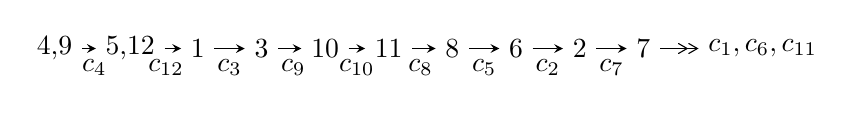
\begin{tikzpicture}[x=23pt, y=7pt]
	% node
	\node (A0) at (-1/8, 0) {4,9};
	\node (A1) at (17/16, 0) {5,12};
	\node (A2) at (17/8, 0) {1};
	\node (A3) at (25/8, 0) {3};
	\node (A4) at (33/8, 0) {10};
	\node (A5) at (41/8, 0) {11};
	\node (A6) at (49/8, 0) {8};
	\node (A7) at (57/8, 0) {6};
	\node (A8) at (65/8, 0) {2};
	\node (A9) at (73/8, 0) {7};
	\node (C1) at (1/2, -1) {$c_{4}$};
	\node (C2) at (13/8, -1) {$c_{12}$};
	\node (C3) at (21/8, -1) {$c_{3}$};
	\node (C4) at (29/8, -1) {$c_{9}$};
	\node (C5) at (37/8, -1) {$c_{10}$};
	\node (C6) at (45/8, -1) {$c_{8}$};
	\node (C7) at (53/8, -1) {$c_{5}$};
	\node (C8) at (61/8, -1) {$c_{2}$};
	\node (C9) at (69/8, -1) {$c_{7}$};
	\node (A10) at (11, 0) {$c_{1},c_{6},c_{11}$};

	% edge
	\draw[->,>=stealth]	
	(A0) edge (A1) (A1) edge (A2) (A2) edge (A3) (A3) edge (A4) (A4) edge (A5) (A5) edge (A6) (A6) edge (A7) (A7) edge (A8) (A8) edge (A9) ;
	\draw[->>,>={angle 60}]	
	(A9) edge (A10);
\end{tikzpicture} \\ 

\end{tabular} \\

\footnotetext{
The image of knot diagram is generated by the software ``\textbf{Draw programme}" developed by Andrew Bartholomew(\url{http://www.layer8.co.uk/maths/draw/index.htm\#Running-draw}), where we modified some parts for our purpose(\url{https://github.com/CATsTAILs/LinksPainter}).
}\phantom \\ \newline 
\centering \textbf{Ideals for irreducible components\footnotemark of $X_{\text{par}}$} 
 
\begin{align*}
I^u_{1}&=\langle 
1096 u^{18}+7571 u^{17}+\cdots+2606 b+15844,\;3961 u^{18}+29496 u^{17}+\cdots+5212 a+60062,\\
\phantom{I^u_{1}}&\phantom{= \langle  }u^{19}+8 u^{18}+\cdots+40 u+8\rangle \\
I^u_{2}&=\langle 
u^{22}-7 u^{21}+\cdots+4 b-16,\;-80 u^{22} a+97 u^{22}+\cdots-45 a+3,\;u^{23}-3 u^{22}+\cdots-11 u+5\rangle \\
I^u_{3}&=\langle 
u^9- u^8+5 u^7-5 u^6+9 u^5-7 u^4+7 u^3-2 u^2+b+u,\;u^8- u^7+5 u^6-5 u^5+9 u^4-7 u^3+7 u^2+a-2 u+1,\\
\phantom{I^u_{3}}&\phantom{= \langle  }u^{10}- u^9+6 u^8-5 u^7+13 u^6-7 u^5+12 u^4- u^3+4 u^2+2 u+1\rangle \\
I^u_{4}&=\langle 
a u+b+1,\;u^4 a+u^4+3 u^2 a+a^2+4 u^2+2 a+4,\;u^5+3 u^3+2 u-1\rangle \\
\\
\end{align*}
\raggedright * 4 irreducible components of $\dim_{\mathbb{C}}=0$, with total 85 representations.\\
\footnotetext{All coefficients of polynomials are rational numbers. But the coefficients are sometimes approximated in decimal forms when there is not enough margin.}
\newpage
\renewcommand{\arraystretch}{1}
\centering \section*{I. $I^u_{1}= \langle 1096 u^{18}+7571 u^{17}+\cdots+2606 b+15844,\;3961 u^{18}+29496 u^{17}+\cdots+5212 a+60062,\;u^{19}+8 u^{18}+\cdots+40 u+8 \rangle$}
\flushleft \textbf{(i) Arc colorings}\\
\begin{tabular}{m{7pt} m{180pt} m{7pt} m{180pt} }
\flushright $a_{4}=$&$\begin{pmatrix}1\\0\end{pmatrix}$ \\
\flushright $a_{9}=$&$\begin{pmatrix}0\\u\end{pmatrix}$ \\
\flushright $a_{5}=$&$\begin{pmatrix}1\\u^2\end{pmatrix}$ \\
\flushright $a_{12}=$&$\begin{pmatrix}-0.759977 u^{18}-5.65925 u^{17}+\cdots-37.0253 u-11.5238\\-0.420568 u^{18}-2.90522 u^{17}+\cdots-18.8753 u-6.07982\end{pmatrix}$ \\
\flushright $a_{1}=$&$\begin{pmatrix}-0.759977 u^{18}-5.65925 u^{17}+\cdots-37.0253 u-11.5238\\-0.879893 u^{18}-5.90982 u^{17}+\cdots-29.6182 u-9.44436\end{pmatrix}$ \\
\flushright $a_{3}=$&$\begin{pmatrix}-1.19052 u^{18}-8.97371 u^{17}+\cdots-54.1759 u-15.1274\\-0.550460 u^{18}-4.31504 u^{17}+\cdots-31.4935 u-9.52417\end{pmatrix}$ \\
\flushright $a_{10}=$&$\begin{pmatrix}1.44561 u^{18}+10.7231 u^{17}+\cdots+56.3331 u+15.2068\\0.930353 u^{18}+7.22487 u^{17}+\cdots+56.1117 u+15.9685\end{pmatrix}$ \\
\flushright $a_{11}=$&$\begin{pmatrix}0.640061 u^{18}+4.65867 u^{17}+\cdots+21.6825 u+6.60322\\0.550460 u^{18}+4.31504 u^{17}+\cdots+32.4935 u+9.52417\end{pmatrix}$ \\
\flushright $a_{8}=$&$\begin{pmatrix}u\\u^3+u\end{pmatrix}$ \\
\flushright $a_{6}=$&$\begin{pmatrix}u^2+1\\u^4+2 u^2\end{pmatrix}$ \\
\flushright $a_{2}=$&$\begin{pmatrix}-0.399079 u^{18}-3.11992 u^{17}+\cdots-23.7630 u-7.95165\\-0.129893 u^{18}-0.909823 u^{17}+\cdots-2.11819 u-1.44436\end{pmatrix}$ \\
\flushright $a_{7}=$&$\begin{pmatrix}0.879029 u^{18}+6.38162 u^{17}+\cdots+29.0679 u+7.33653\\-0.118764 u^{18}-0.712970 u^{17}+\cdots+2.14083 u+1.38987\end{pmatrix}$\\&\end{tabular}
\flushleft \textbf{(ii) Obstruction class $= -1$}\\~\\
\flushleft \textbf{(iii) Cusp Shapes $= \frac{3773}{1303} u^{18}+\frac{27698}{1303} u^{17}+\cdots+\frac{165236}{1303} u+\frac{31950}{1303}$}\\~\\
\newpage\renewcommand{\arraystretch}{1}
\flushleft \textbf{(iv) u-Polynomials at the component}\newline \\
\begin{tabular}{m{50pt}|m{274pt}}
Crossings & \hspace{64pt}u-Polynomials at each crossing \\
\hline $$\begin{aligned}c_{1},c_{10}\end{aligned}$$&$\begin{aligned}
&u^{19}+11 u^{18}+\cdots-9 u-1
\end{aligned}$\\
\hline $$\begin{aligned}c_{2},c_{6},c_{7}\\c_{11}\end{aligned}$$&$\begin{aligned}
&u^{19}- u^{18}+\cdots- u+1
\end{aligned}$\\
\hline $$\begin{aligned}c_{3},c_{12}\end{aligned}$$&$\begin{aligned}
&u^{19}- u^{18}+\cdots+2 u+1
\end{aligned}$\\
\hline $$\begin{aligned}c_{4},c_{5},c_{8}\end{aligned}$$&$\begin{aligned}
&u^{19}-8 u^{18}+\cdots+40 u-8
\end{aligned}$\\
\hline $$\begin{aligned}c_{9}\end{aligned}$$&$\begin{aligned}
&u^{19}+17 u^{18}+\cdots+672 u+64
\end{aligned}$\\
\hline
\end{tabular}\\~\\
\newpage\renewcommand{\arraystretch}{1}
\flushleft \textbf{(v) Riley Polynomials at the component}\newline \\
\begin{tabular}{m{50pt}|m{274pt}}
Crossings & \hspace{64pt}Riley Polynomials at each crossing \\
\hline $$\begin{aligned}c_{1},c_{10}\end{aligned}$$&$\begin{aligned}
&y^{19}+3 y^{18}+\cdots-5 y-1
\end{aligned}$\\
\hline $$\begin{aligned}c_{2},c_{6},c_{7}\\c_{11}\end{aligned}$$&$\begin{aligned}
&y^{19}+11 y^{18}+\cdots-9 y-1
\end{aligned}$\\
\hline $$\begin{aligned}c_{3},c_{12}\end{aligned}$$&$\begin{aligned}
&y^{19}-25 y^{18}+\cdots-8 y-1
\end{aligned}$\\
\hline $$\begin{aligned}c_{4},c_{5},c_{8}\end{aligned}$$&$\begin{aligned}
&y^{19}+16 y^{18}+\cdots+32 y-64
\end{aligned}$\\
\hline $$\begin{aligned}c_{9}\end{aligned}$$&$\begin{aligned}
&y^{19}-9 y^{18}+\cdots-7168 y-4096
\end{aligned}$\\
\hline
\end{tabular}\\~\\
\newpage\flushleft \textbf{(vi) Complex Volumes and Cusp Shapes}
$$\begin{array}{c|c|c}  
\text{Solutions to }I^u_{1}& \I (\text{vol} + \sqrt{-1}CS) & \text{Cusp shape}\\
 \hline 
\begin{aligned}
u &= -0.616811 + 0.855089 I \\
a &= -1.021840 - 0.627553 I \\
b &= -1.166890 + 0.486679 I\end{aligned}
 & -3.17455 + 2.33222 I & -9.09826 - 1.94044 I \\ \hline\begin{aligned}
u &= -0.616811 - 0.855089 I \\
a &= -1.021840 + 0.627553 I \\
b &= -1.166890 - 0.486679 I\end{aligned}
 & -3.17455 - 2.33222 I & -9.09826 + 1.94044 I \\ \hline\begin{aligned}
u &= -1.120010 + 0.195383 I \\
a &= \phantom{-}1.52958 + 0.02914 I \\
b &= \phantom{-}1.71883 - 0.26621 I\end{aligned}
 & -9.12103 + 9.62063 I & -8.08284 - 6.41226 I \\ \hline\begin{aligned}
u &= -1.120010 - 0.195383 I \\
a &= \phantom{-}1.52958 - 0.02914 I \\
b &= \phantom{-}1.71883 + 0.26621 I\end{aligned}
 & -9.12103 - 9.62063 I & -8.08284 + 6.41226 I \\ \hline\begin{aligned}
u &= -0.678394 + 0.473924 I \\
a &= -0.638948 - 0.805280 I \\
b &= -0.815100 - 0.243485 I\end{aligned}
 & -3.94120 + 2.37372 I & -9.61488 - 3.89895 I \\ \hline\begin{aligned}
u &= -0.678394 - 0.473924 I \\
a &= -0.638948 + 0.805280 I \\
b &= -0.815100 + 0.243485 I\end{aligned}
 & -3.94120 - 2.37372 I & -9.61488 + 3.89895 I \\ \hline\begin{aligned}
u &= -0.643620\phantom{ +0.000000I} \\
a &= -2.20220\phantom{ +0.000000I} \\
b &= -1.41738\phantom{ +0.000000I}\end{aligned}
 & -2.91062\phantom{ +0.000000I} & -2.04050\phantom{ +0.000000I} \\ \hline\begin{aligned}
u &= -0.283257 + 1.330640 I \\
a &= -0.629985 - 0.965924 I \\
b &= -1.46374 + 0.56468 I\end{aligned}
 & \phantom{-}1.36748 + 3.35758 I & -0.130533 - 0.838590 I \\ \hline\begin{aligned}
u &= -0.283257 - 1.330640 I \\
a &= -0.629985 + 0.965924 I \\
b &= -1.46374 - 0.56468 I\end{aligned}
 & \phantom{-}1.36748 - 3.35758 I & -0.130533 + 0.838590 I \\ \hline\begin{aligned}
u &= -0.72609 + 1.25708 I \\
a &= \phantom{-}0.602034 + 0.850739 I \\
b &= \phantom{-}1.50658 - 0.13910 I\end{aligned}
 & -5.96103 - 3.19218 I & -6.11033 + 3.75659 I\\
 \hline 
 \end{array}$$\newpage$$\begin{array}{c|c|c}  
\text{Solutions to }I^u_{1}& \I (\text{vol} + \sqrt{-1}CS) & \text{Cusp shape}\\
 \hline 
\begin{aligned}
u &= -0.72609 - 1.25708 I \\
a &= \phantom{-}0.602034 - 0.850739 I \\
b &= \phantom{-}1.50658 + 0.13910 I\end{aligned}
 & -5.96103 + 3.19218 I & -6.11033 - 3.75659 I \\ \hline\begin{aligned}
u &= \phantom{-}0.344998 + 0.346579 I \\
a &= \phantom{-}0.494258 + 0.345842 I \\
b &= -0.050657 - 0.290614 I\end{aligned}
 & -0.136375 - 0.955727 I & -2.79406 + 6.93579 I \\ \hline\begin{aligned}
u &= \phantom{-}0.344998 - 0.346579 I \\
a &= \phantom{-}0.494258 - 0.345842 I \\
b &= -0.050657 + 0.290614 I\end{aligned}
 & -0.136375 + 0.955727 I & -2.79406 - 6.93579 I \\ \hline\begin{aligned}
u &= -0.20896 + 1.50540 I \\
a &= \phantom{-}0.164518 - 0.451521 I \\
b &= -0.645343 - 0.342017 I\end{aligned}
 & \phantom{-}2.53796 + 5.54235 I & -7.14543 - 3.27743 I \\ \hline\begin{aligned}
u &= -0.20896 - 1.50540 I \\
a &= \phantom{-}0.164518 + 0.451521 I \\
b &= -0.645343 + 0.342017 I\end{aligned}
 & \phantom{-}2.53796 - 5.54235 I & -7.14543 + 3.27743 I \\ \hline\begin{aligned}
u &= -0.49084 + 1.46047 I \\
a &= \phantom{-}0.735940 + 0.906077 I \\
b &= \phantom{-}1.68453 - 0.63008 I\end{aligned}
 & -3.8953 + 15.3465 I & -4.88591 - 8.00097 I \\ \hline\begin{aligned}
u &= -0.49084 - 1.46047 I \\
a &= \phantom{-}0.735940 - 0.906077 I \\
b &= \phantom{-}1.68453 + 0.63008 I\end{aligned}
 & -3.8953 - 15.3465 I & -4.88591 + 8.00097 I \\ \hline\begin{aligned}
u &= \phantom{-}0.10117 + 1.56824 I \\
a &= \phantom{-}0.115543 + 0.288337 I \\
b &= \phantom{-}0.440490 - 0.210371 I\end{aligned}
 & \phantom{-}6.50755 - 2.80738 I & -1.61751 + 0.28698 I \\ \hline\begin{aligned}
u &= \phantom{-}0.10117 - 1.56824 I \\
a &= \phantom{-}0.115543 - 0.288337 I \\
b &= \phantom{-}0.440490 + 0.210371 I\end{aligned}
 & \phantom{-}6.50755 + 2.80738 I & -1.61751 - 0.28698 I\\
 \hline 
 \end{array}$$\newpage\newpage\renewcommand{\arraystretch}{1}
\centering \section*{II. $I^u_{2}= \langle u^{22}-7 u^{21}+\cdots+4 b-16,\;-80 u^{22} a+97 u^{22}+\cdots-45 a+3,\;u^{23}-3 u^{22}+\cdots-11 u+5 \rangle$}
\flushleft \textbf{(i) Arc colorings}\\
\begin{tabular}{m{7pt} m{180pt} m{7pt} m{180pt} }
\flushright $a_{4}=$&$\begin{pmatrix}1\\0\end{pmatrix}$ \\
\flushright $a_{9}=$&$\begin{pmatrix}0\\u\end{pmatrix}$ \\
\flushright $a_{5}=$&$\begin{pmatrix}1\\u^2\end{pmatrix}$ \\
\flushright $a_{12}=$&$\begin{pmatrix}a\\-\frac{1}{4} u^{22}+\frac{7}{4} u^{21}+\cdots-\frac{37}{4} u+4\end{pmatrix}$ \\
\flushright $a_{1}=$&$\begin{pmatrix}a\\-\frac{1}{4} u^{22}+\frac{7}{4} u^{21}+\cdots-\frac{37}{4} u+4\end{pmatrix}$ \\
\flushright $a_{3}=$&$\begin{pmatrix}0.350000 u^{22}-2.05000 u^{21}+\cdots+10.7000 u-3.85000\\- u^{22} a-\frac{7}{4} u^{22}+\cdots-\frac{5}{4} a+\frac{29}{4}\end{pmatrix}$ \\
\flushright $a_{10}=$&$\begin{pmatrix}0.0500000 u^{22}-1.15000 u^{21}+\cdots+8.35000 u-4.55000\\\frac{3}{2} u^{22} a-\frac{3}{2} u^{22}+\cdots-\frac{15}{4} a-\frac{13}{4}\end{pmatrix}$ \\
\flushright $a_{11}=$&$\begin{pmatrix}-\frac{1}{4} u^{22} a+\frac{27}{20} u^{22}+\cdots+4 a-\frac{31}{10}\\- u^{22}+\frac{9}{4} u^{21}+\cdots+\frac{33}{4} u^2-\frac{7}{4}\end{pmatrix}$ \\
\flushright $a_{8}=$&$\begin{pmatrix}u\\u^3+u\end{pmatrix}$ \\
\flushright $a_{6}=$&$\begin{pmatrix}u^2+1\\u^4+2 u^2\end{pmatrix}$ \\
\flushright $a_{2}=$&$\begin{pmatrix}\frac{1}{2} u^{21} a+\frac{11}{10} u^{22}+\cdots+\frac{5}{2} a-\frac{97}{20}\\-\frac{1}{2} u^{22} a- u^{22}+\cdots-7 u+1\end{pmatrix}$ \\
\flushright $a_{7}=$&$\begin{pmatrix}\frac{3}{4} u^{22} a+\frac{13}{20} u^{22}+\cdots-2 a-\frac{29}{10}\\\frac{3}{4} u^{22} a+\frac{1}{2} u^{22}+\cdots+\frac{5}{4} a-4\end{pmatrix}$\\&\end{tabular}
\flushleft \textbf{(ii) Obstruction class $= -1$}\\~\\
\flushleft \textbf{(iii) Cusp Shapes $= 2 u^{21}-5 u^{20}+25 u^{19}-48 u^{18}+126 u^{17}-191 u^{16}+333 u^{15}-398 u^{14}+484 u^{13}-437 u^{12}+341 u^{11}-191 u^{10}+29 u^9+56 u^8-78 u^7+72 u^6+8 u^5+13 u^4+23 u^3+6 u^2-8 u-2$}\\~\\
\newpage\renewcommand{\arraystretch}{1}
\flushleft \textbf{(iv) u-Polynomials at the component}\newline \\
\begin{tabular}{m{50pt}|m{274pt}}
Crossings & \hspace{64pt}u-Polynomials at each crossing \\
\hline $$\begin{aligned}c_{1},c_{10}\end{aligned}$$&$\begin{aligned}
&u^{46}+26 u^{45}+\cdots+2067 u+121
\end{aligned}$\\
\hline $$\begin{aligned}c_{2},c_{6},c_{7}\\c_{11}\end{aligned}$$&$\begin{aligned}
&u^{46}-2 u^{45}+\cdots-45 u+11
\end{aligned}$\\
\hline $$\begin{aligned}c_{3},c_{12}\end{aligned}$$&$\begin{aligned}
&u^{46}-2 u^{45}+\cdots+117 u+7
\end{aligned}$\\
\hline $$\begin{aligned}c_{4},c_{5},c_{8}\end{aligned}$$&$\begin{aligned}
&(u^{23}+3 u^{22}+\cdots-11 u-5)^{2}
\end{aligned}$\\
\hline $$\begin{aligned}c_{9}\end{aligned}$$&$\begin{aligned}
&(u^{23}-8 u^{22}+\cdots-26 u+5)^{2}
\end{aligned}$\\
\hline
\end{tabular}\\~\\
\newpage\renewcommand{\arraystretch}{1}
\flushleft \textbf{(v) Riley Polynomials at the component}\newline \\
\begin{tabular}{m{50pt}|m{274pt}}
Crossings & \hspace{64pt}Riley Polynomials at each crossing \\
\hline $$\begin{aligned}c_{1},c_{10}\end{aligned}$$&$\begin{aligned}
&y^{46}-6 y^{45}+\cdots-691857 y+14641
\end{aligned}$\\
\hline $$\begin{aligned}c_{2},c_{6},c_{7}\\c_{11}\end{aligned}$$&$\begin{aligned}
&y^{46}+26 y^{45}+\cdots+2067 y+121
\end{aligned}$\\
\hline $$\begin{aligned}c_{3},c_{12}\end{aligned}$$&$\begin{aligned}
&y^{46}-42 y^{45}+\cdots+4707 y+49
\end{aligned}$\\
\hline $$\begin{aligned}c_{4},c_{5},c_{8}\end{aligned}$$&$\begin{aligned}
&(y^{23}+21 y^{22}+\cdots+51 y-25)^{2}
\end{aligned}$\\
\hline $$\begin{aligned}c_{9}\end{aligned}$$&$\begin{aligned}
&(y^{23}-32 y^{22}+\cdots+36 y-25)^{2}
\end{aligned}$\\
\hline
\end{tabular}\\~\\
\newpage\flushleft \textbf{(vi) Complex Volumes and Cusp Shapes}
$$\begin{array}{c|c|c}  
\text{Solutions to }I^u_{2}& \I (\text{vol} + \sqrt{-1}CS) & \text{Cusp shape}\\
 \hline 
\begin{aligned}
u &= \phantom{-}0.949457 + 0.274301 I \\
a &= -1.53072 + 0.32112 I \\
b &= -1.70279 - 0.29302 I\end{aligned}
 & -6.21980 - 4.08700 I & -6.45479 + 3.28019 I \\ \hline\begin{aligned}
u &= \phantom{-}0.949457 + 0.274301 I \\
a &= \phantom{-}1.73757 - 0.19337 I \\
b &= \phantom{-}1.54144 + 0.11499 I\end{aligned}
 & -6.21980 - 4.08700 I & -6.45479 + 3.28019 I \\ \hline\begin{aligned}
u &= \phantom{-}0.949457 - 0.274301 I \\
a &= -1.53072 - 0.32112 I \\
b &= -1.70279 + 0.29302 I\end{aligned}
 & -6.21980 + 4.08700 I & -6.45479 - 3.28019 I \\ \hline\begin{aligned}
u &= \phantom{-}0.949457 - 0.274301 I \\
a &= \phantom{-}1.73757 + 0.19337 I \\
b &= \phantom{-}1.54144 - 0.11499 I\end{aligned}
 & -6.21980 + 4.08700 I & -6.45479 - 3.28019 I \\ \hline\begin{aligned}
u &= \phantom{-}0.129915 + 1.043420 I \\
a &= -0.493058 + 0.848090 I \\
b &= -1.94953 - 0.23067 I\end{aligned}
 & -5.55917 - 0.57299 I & -3.52244 - 2.34138 I \\ \hline\begin{aligned}
u &= \phantom{-}0.129915 + 1.043420 I \\
a &= \phantom{-}0.44678 - 1.81277 I \\
b &= \phantom{-}0.948973 + 0.404288 I\end{aligned}
 & -5.55917 - 0.57299 I & -3.52244 - 2.34138 I \\ \hline\begin{aligned}
u &= \phantom{-}0.129915 - 1.043420 I \\
a &= -0.493058 - 0.848090 I \\
b &= -1.94953 + 0.23067 I\end{aligned}
 & -5.55917 + 0.57299 I & -3.52244 + 2.34138 I \\ \hline\begin{aligned}
u &= \phantom{-}0.129915 - 1.043420 I \\
a &= \phantom{-}0.44678 + 1.81277 I \\
b &= \phantom{-}0.948973 - 0.404288 I\end{aligned}
 & -5.55917 + 0.57299 I & -3.52244 + 2.34138 I \\ \hline\begin{aligned}
u &= \phantom{-}0.157565 + 1.169780 I \\
a &= \phantom{-}0.170495 - 0.884679 I \\
b &= -0.525087 + 1.299010 I\end{aligned}
 & \phantom{-}2.81400 - 1.37485 I & -2.47637 + 0.94605 I \\ \hline\begin{aligned}
u &= \phantom{-}0.157565 + 1.169780 I \\
a &= -1.031300 - 0.587788 I \\
b &= -1.061750 - 0.060047 I\end{aligned}
 & \phantom{-}2.81400 - 1.37485 I & -2.47637 + 0.94605 I\\
 \hline 
 \end{array}$$\newpage$$\begin{array}{c|c|c}  
\text{Solutions to }I^u_{2}& \I (\text{vol} + \sqrt{-1}CS) & \text{Cusp shape}\\
 \hline 
\begin{aligned}
u &= \phantom{-}0.157565 - 1.169780 I \\
a &= \phantom{-}0.170495 + 0.884679 I \\
b &= -0.525087 - 1.299010 I\end{aligned}
 & \phantom{-}2.81400 + 1.37485 I & -2.47637 - 0.94605 I \\ \hline\begin{aligned}
u &= \phantom{-}0.157565 - 1.169780 I \\
a &= -1.031300 + 0.587788 I \\
b &= -1.061750 + 0.060047 I\end{aligned}
 & \phantom{-}2.81400 + 1.37485 I & -2.47637 - 0.94605 I \\ \hline\begin{aligned}
u &= -0.297704 + 1.164290 I \\
a &= -0.315648 - 0.681415 I \\
b &= \phantom{-}0.02755 + 1.63095 I\end{aligned}
 & \phantom{-}1.67762 + 7.26897 I & -4.60706 - 6.86727 I \\ \hline\begin{aligned}
u &= -0.297704 + 1.164290 I \\
a &= -1.309170 + 0.358408 I \\
b &= -0.887336 + 0.164646 I\end{aligned}
 & \phantom{-}1.67762 + 7.26897 I & -4.60706 - 6.86727 I \\ \hline\begin{aligned}
u &= -0.297704 - 1.164290 I \\
a &= -0.315648 + 0.681415 I \\
b &= \phantom{-}0.02755 - 1.63095 I\end{aligned}
 & \phantom{-}1.67762 - 7.26897 I & -4.60706 + 6.86727 I \\ \hline\begin{aligned}
u &= -0.297704 - 1.164290 I \\
a &= -1.309170 - 0.358408 I \\
b &= -0.887336 - 0.164646 I\end{aligned}
 & \phantom{-}1.67762 - 7.26897 I & -4.60706 + 6.86727 I \\ \hline\begin{aligned}
u &= \phantom{-}0.701104 + 1.024510 I \\
a &= -0.679056 + 0.799381 I \\
b &= -1.62187 - 0.29006 I\end{aligned}
 & -4.06293 - 1.56405 I & -5.53705 + 2.00718 I \\ \hline\begin{aligned}
u &= \phantom{-}0.701104 + 1.024510 I \\
a &= \phantom{-}0.930638 - 0.946208 I \\
b &= \phantom{-}1.295060 + 0.135249 I\end{aligned}
 & -4.06293 - 1.56405 I & -5.53705 + 2.00718 I \\ \hline\begin{aligned}
u &= \phantom{-}0.701104 - 1.024510 I \\
a &= -0.679056 - 0.799381 I \\
b &= -1.62187 + 0.29006 I\end{aligned}
 & -4.06293 + 1.56405 I & -5.53705 - 2.00718 I \\ \hline\begin{aligned}
u &= \phantom{-}0.701104 - 1.024510 I \\
a &= \phantom{-}0.930638 + 0.946208 I \\
b &= \phantom{-}1.295060 - 0.135249 I\end{aligned}
 & -4.06293 + 1.56405 I & -5.53705 - 2.00718 I\\
 \hline 
 \end{array}$$\newpage$$\begin{array}{c|c|c}  
\text{Solutions to }I^u_{2}& \I (\text{vol} + \sqrt{-1}CS) & \text{Cusp shape}\\
 \hline 
\begin{aligned}
u &= -0.700899\phantom{ +0.000000I} \\
a &= \phantom{-}2.31801 + 0.38865 I \\
b &= \phantom{-}1.62469 - 0.27240 I\end{aligned}
 & -11.2801\phantom{ +0.000000I} & -11.1210\phantom{ +0.000000I} \\ \hline\begin{aligned}
u &= -0.700899\phantom{ +0.000000I} \\
a &= \phantom{-}2.31801 - 0.38865 I \\
b &= \phantom{-}1.62469 + 0.27240 I\end{aligned}
 & -11.2801\phantom{ +0.000000I} & -11.1210\phantom{ +0.000000I} \\ \hline\begin{aligned}
u &= \phantom{-}0.098502 + 1.344050 I \\
a &= \phantom{-}0.866199 - 0.095805 I \\
b &= \phantom{-}0.845917 - 0.031157 I\end{aligned}
 & \phantom{-}5.30060 - 3.06078 I & \phantom{-}0.29039 + 3.85817 I \\ \hline\begin{aligned}
u &= \phantom{-}0.098502 + 1.344050 I \\
a &= -0.022822 + 0.627708 I \\
b &= -0.214088 - 1.154780 I\end{aligned}
 & \phantom{-}5.30060 - 3.06078 I & \phantom{-}0.29039 + 3.85817 I \\ \hline\begin{aligned}
u &= \phantom{-}0.098502 - 1.344050 I \\
a &= \phantom{-}0.866199 + 0.095805 I \\
b &= \phantom{-}0.845917 + 0.031157 I\end{aligned}
 & \phantom{-}5.30060 + 3.06078 I & \phantom{-}0.29039 - 3.85817 I \\ \hline\begin{aligned}
u &= \phantom{-}0.098502 - 1.344050 I \\
a &= -0.022822 - 0.627708 I \\
b &= -0.214088 + 1.154780 I\end{aligned}
 & \phantom{-}5.30060 + 3.06078 I & \phantom{-}0.29039 - 3.85817 I \\ \hline\begin{aligned}
u &= -0.314282 + 1.335820 I \\
a &= \phantom{-}0.636808 + 0.819242 I \\
b &= \phantom{-}1.79937 - 0.02411 I\end{aligned}
 & -7.00942 + 3.66737 I & -5.63248 - 4.77182 I \\ \hline\begin{aligned}
u &= -0.314282 + 1.335820 I \\
a &= \phantom{-}0.317399 + 1.272340 I \\
b &= \phantom{-}1.29450 - 0.59319 I\end{aligned}
 & -7.00942 + 3.66737 I & -5.63248 - 4.77182 I \\ \hline\begin{aligned}
u &= -0.314282 - 1.335820 I \\
a &= \phantom{-}0.636808 - 0.819242 I \\
b &= \phantom{-}1.79937 + 0.02411 I\end{aligned}
 & -7.00942 - 3.66737 I & -5.63248 + 4.77182 I \\ \hline\begin{aligned}
u &= -0.314282 - 1.335820 I \\
a &= \phantom{-}0.317399 - 1.272340 I \\
b &= \phantom{-}1.29450 + 0.59319 I\end{aligned}
 & -7.00942 - 3.66737 I & -5.63248 + 4.77182 I\\
 \hline 
 \end{array}$$\newpage$$\begin{array}{c|c|c}  
\text{Solutions to }I^u_{2}& \I (\text{vol} + \sqrt{-1}CS) & \text{Cusp shape}\\
 \hline 
\begin{aligned}
u &= -0.540846 + 0.315918 I \\
a &= \phantom{-}0.051854 - 0.150163 I \\
b &= -0.539179 - 1.227400 I\end{aligned}
 & -0.93518 - 3.99671 I & -9.62845 + 1.40973 I \\ \hline\begin{aligned}
u &= -0.540846 + 0.315918 I \\
a &= \phantom{-}0.24507 - 2.12626 I \\
b &= -0.0193942 - 0.0975969 I\end{aligned}
 & -0.93518 - 3.99671 I & -9.62845 + 1.40973 I \\ \hline\begin{aligned}
u &= -0.540846 - 0.315918 I \\
a &= \phantom{-}0.051854 + 0.150163 I \\
b &= -0.539179 + 1.227400 I\end{aligned}
 & -0.93518 + 3.99671 I & -9.62845 - 1.40973 I \\ \hline\begin{aligned}
u &= -0.540846 - 0.315918 I \\
a &= \phantom{-}0.24507 + 2.12626 I \\
b &= -0.0193942 + 0.0975969 I\end{aligned}
 & -0.93518 + 3.99671 I & -9.62845 - 1.40973 I \\ \hline\begin{aligned}
u &= \phantom{-}0.499495 + 0.232325 I \\
a &= \phantom{-}0.80490 + 1.31816 I \\
b &= -0.0999299 - 0.0558064 I\end{aligned}
 & \phantom{-}0.125631 - 0.991368 I & -5.18428 + 5.58556 I \\ \hline\begin{aligned}
u &= \phantom{-}0.499495 + 0.232325 I \\
a &= \phantom{-}0.207202 + 0.015352 I \\
b &= -0.095801 - 0.845413 I\end{aligned}
 & \phantom{-}0.125631 - 0.991368 I & -5.18428 + 5.58556 I \\ \hline\begin{aligned}
u &= \phantom{-}0.499495 - 0.232325 I \\
a &= \phantom{-}0.80490 - 1.31816 I \\
b &= -0.0999299 + 0.0558064 I\end{aligned}
 & \phantom{-}0.125631 + 0.991368 I & -5.18428 - 5.58556 I \\ \hline\begin{aligned}
u &= \phantom{-}0.499495 - 0.232325 I \\
a &= \phantom{-}0.207202 - 0.015352 I \\
b &= -0.095801 + 0.845413 I\end{aligned}
 & \phantom{-}0.125631 + 0.991368 I & -5.18428 - 5.58556 I \\ \hline\begin{aligned}
u &= \phantom{-}0.40672 + 1.44182 I \\
a &= -0.563943 + 0.961951 I \\
b &= -1.54904 - 0.71550 I\end{aligned}
 & -0.79781 - 8.96070 I & -2.64189 + 5.31157 I \\ \hline\begin{aligned}
u &= \phantom{-}0.40672 + 1.44182 I \\
a &= \phantom{-}0.740402 - 0.865507 I \\
b &= \phantom{-}1.61633 + 0.42186 I\end{aligned}
 & -0.79781 - 8.96070 I & -2.64189 + 5.31157 I\\
 \hline 
 \end{array}$$\newpage$$\begin{array}{c|c|c}  
\text{Solutions to }I^u_{2}& \I (\text{vol} + \sqrt{-1}CS) & \text{Cusp shape}\\
 \hline 
\begin{aligned}
u &= \phantom{-}0.40672 - 1.44182 I \\
a &= -0.563943 - 0.961951 I \\
b &= -1.54904 + 0.71550 I\end{aligned}
 & -0.79781 + 8.96070 I & -2.64189 - 5.31157 I \\ \hline\begin{aligned}
u &= \phantom{-}0.40672 - 1.44182 I \\
a &= \phantom{-}0.740402 + 0.865507 I \\
b &= \phantom{-}1.61633 - 0.42186 I\end{aligned}
 & -0.79781 + 8.96070 I & -2.64189 - 5.31157 I \\ \hline\begin{aligned}
u &= \phantom{-}0.06052 + 1.52562 I \\
a &= \phantom{-}0.443758 - 0.312131 I \\
b &= \phantom{-}0.775017 - 0.227308 I\end{aligned}
 & \phantom{-}5.50209 - 2.76341 I & -4.54493 + 5.66390 I \\ \hline\begin{aligned}
u &= \phantom{-}0.06052 + 1.52562 I \\
a &= \phantom{-}0.128639 + 0.513106 I \\
b &= -0.503049 - 0.658113 I\end{aligned}
 & \phantom{-}5.50209 - 2.76341 I & -4.54493 + 5.66390 I \\ \hline\begin{aligned}
u &= \phantom{-}0.06052 - 1.52562 I \\
a &= \phantom{-}0.443758 + 0.312131 I \\
b &= \phantom{-}0.775017 + 0.227308 I\end{aligned}
 & \phantom{-}5.50209 + 2.76341 I & -4.54493 - 5.66390 I \\ \hline\begin{aligned}
u &= \phantom{-}0.06052 - 1.52562 I \\
a &= \phantom{-}0.128639 - 0.513106 I \\
b &= -0.503049 + 0.658113 I\end{aligned}
 & \phantom{-}5.50209 + 2.76341 I & -4.54493 - 5.66390 I\\
 \hline 
 \end{array}$$\newpage\newpage\renewcommand{\arraystretch}{1}
\centering \section*{III. $I^u_{3}= \langle u^9- u^8+\cdots+b+u,\;u^8- u^7+\cdots+a+1,\;u^{10}- u^9+\cdots+2 u+1 \rangle$}
\flushleft \textbf{(i) Arc colorings}\\
\begin{tabular}{m{7pt} m{180pt} m{7pt} m{180pt} }
\flushright $a_{4}=$&$\begin{pmatrix}1\\0\end{pmatrix}$ \\
\flushright $a_{9}=$&$\begin{pmatrix}0\\u\end{pmatrix}$ \\
\flushright $a_{5}=$&$\begin{pmatrix}1\\u^2\end{pmatrix}$ \\
\flushright $a_{12}=$&$\begin{pmatrix}- u^8+u^7-5 u^6+5 u^5-9 u^4+7 u^3-7 u^2+2 u-1\\- u^9+u^8-5 u^7+5 u^6-9 u^5+7 u^4-7 u^3+2 u^2- u\end{pmatrix}$ \\
\flushright $a_{1}=$&$\begin{pmatrix}- u^8+u^7-5 u^6+5 u^5-9 u^4+7 u^3-7 u^2+2 u-1\\- u^9+2 u^8-5 u^7+9 u^6-9 u^5+12 u^4-6 u^3+5 u^2+u+1\end{pmatrix}$ \\
\flushright $a_{3}=$&$\begin{pmatrix}u^8- u^7+5 u^6-4 u^5+8 u^4-3 u^3+4 u^2+2 u\\u^9- u^8+5 u^7-4 u^6+8 u^5-3 u^4+4 u^3+2 u^2- u\end{pmatrix}$ \\
\flushright $a_{10}=$&$\begin{pmatrix}2 u^8- u^7+9 u^6-4 u^5+13 u^4-2 u^3+8 u^2+4 u+2\\2 u^9-2 u^8+10 u^7-9 u^6+17 u^5-10 u^4+11 u^3+u-1\end{pmatrix}$ \\
\flushright $a_{11}=$&$\begin{pmatrix}- u^9+2 u^8-6 u^7+9 u^6-12 u^5+11 u^4-7 u^3+2 u^2+2 u-1\\u^9- u^8+5 u^7-4 u^6+8 u^5-3 u^4+4 u^3+2 u^2\end{pmatrix}$ \\
\flushright $a_{8}=$&$\begin{pmatrix}u\\u^3+u\end{pmatrix}$ \\
\flushright $a_{6}=$&$\begin{pmatrix}u^2+1\\u^4+2 u^2\end{pmatrix}$ \\
\flushright $a_{2}=$&$\begin{pmatrix}u^8- u^7+5 u^6-3 u^5+7 u^4+2 u^2+4 u\\u^9+5 u^7+8 u^5+2 u^4+5 u^3+5 u^2+u+1\end{pmatrix}$ \\
\flushright $a_{7}=$&$\begin{pmatrix}- u^9+u^8-6 u^7+6 u^6-13 u^5+10 u^4-12 u^3+4 u^2-3 u+1\\u^8+4 u^6+5 u^4+2 u^3+3 u^2+4 u+1\end{pmatrix}$\\&\end{tabular}
\flushleft \textbf{(ii) Obstruction class $= 1$}\\~\\
\flushleft \textbf{(iii) Cusp Shapes $= 5 u^9-4 u^8+24 u^7-20 u^6+44 u^5-28 u^4+40 u^3-8 u^2+12 u$}\\~\\
\newpage\renewcommand{\arraystretch}{1}
\flushleft \textbf{(iv) u-Polynomials at the component}\newline \\
\begin{tabular}{m{50pt}|m{274pt}}
Crossings & \hspace{64pt}u-Polynomials at each crossing \\
\hline $$\begin{aligned}c_{1},c_{10}\end{aligned}$$&$\begin{aligned}
&u^{10}-7 u^9+\cdots-8 u+1
\end{aligned}$\\
\hline $$\begin{aligned}c_{2},c_{7}\end{aligned}$$&$\begin{aligned}
&u^{10}- u^9+4 u^8-3 u^7+7 u^6-4 u^5+7 u^4-3 u^3+4 u^2+1
\end{aligned}$\\
\hline $$\begin{aligned}c_{3},c_{12}\end{aligned}$$&$\begin{aligned}
&u^{10}+u^9-2 u^8-4 u^7-3 u^6+u^5+6 u^4+7 u^3+6 u^2+3 u+1
\end{aligned}$\\
\hline $$\begin{aligned}c_{4},c_{5}\end{aligned}$$&$\begin{aligned}
&u^{10}- u^9+6 u^8-5 u^7+13 u^6-7 u^5+12 u^4- u^3+4 u^2+2 u+1
\end{aligned}$\\
\hline $$\begin{aligned}c_{6},c_{11}\end{aligned}$$&$\begin{aligned}
&u^{10}+u^9+4 u^8+3 u^7+7 u^6+4 u^5+7 u^4+3 u^3+4 u^2+1
\end{aligned}$\\
\hline $$\begin{aligned}c_{8}\end{aligned}$$&$\begin{aligned}
&u^{10}+u^9+6 u^8+5 u^7+13 u^6+7 u^5+12 u^4+u^3+4 u^2-2 u+1
\end{aligned}$\\
\hline $$\begin{aligned}c_{9}\end{aligned}$$&$\begin{aligned}
&u^{10}-4 u^9+6 u^8-10 u^7+17 u^6-13 u^5+11 u^4-7 u^3-2 u^2+u+1
\end{aligned}$\\
\hline
\end{tabular}\\~\\
\newpage\renewcommand{\arraystretch}{1}
\flushleft \textbf{(v) Riley Polynomials at the component}\newline \\
\begin{tabular}{m{50pt}|m{274pt}}
Crossings & \hspace{64pt}Riley Polynomials at each crossing \\
\hline $$\begin{aligned}c_{1},c_{10}\end{aligned}$$&$\begin{aligned}
&y^{10}- y^9-19 y^7-21 y^6+34 y^5+145 y^4+217 y^3+102 y^2-4 y+1
\end{aligned}$\\
\hline $$\begin{aligned}c_{2},c_{6},c_{7}\\c_{11}\end{aligned}$$&$\begin{aligned}
&y^{10}+7 y^9+\cdots+8 y+1
\end{aligned}$\\
\hline $$\begin{aligned}c_{3},c_{12}\end{aligned}$$&$\begin{aligned}
&y^{10}-5 y^9+6 y^8+6 y^7-9 y^6-9 y^5+6 y^4+11 y^3+6 y^2+3 y+1
\end{aligned}$\\
\hline $$\begin{aligned}c_{4},c_{5},c_{8}\end{aligned}$$&$\begin{aligned}
&y^{10}+11 y^9+\cdots+4 y+1
\end{aligned}$\\
\hline $$\begin{aligned}c_{9}\end{aligned}$$&$\begin{aligned}
&y^{10}-4 y^9+\cdots-5 y+1
\end{aligned}$\\
\hline
\end{tabular}\\~\\
\newpage\flushleft \textbf{(vi) Complex Volumes and Cusp Shapes}
$$\begin{array}{c|c|c}  
\text{Solutions to }I^u_{3}& \I (\text{vol} + \sqrt{-1}CS) & \text{Cusp shape}\\
 \hline 
\begin{aligned}
u &= \phantom{-}0.250000 + 0.998657 I \\
a &= \phantom{-}0.59595 - 1.38352 I \\
b &= \phantom{-}1.53065 + 0.24927 I\end{aligned}
 & -8.30263 - 0.98508 I & -8.00878 + 0.35212 I \\ \hline\begin{aligned}
u &= \phantom{-}0.250000 - 0.998657 I \\
a &= \phantom{-}0.59595 + 1.38352 I \\
b &= \phantom{-}1.53065 - 0.24927 I\end{aligned}
 & -8.30263 + 0.98508 I & -8.00878 - 0.35212 I \\ \hline\begin{aligned}
u &= \phantom{-}0.692359 + 0.857180 I \\
a &= -0.929090 + 0.709584 I \\
b &= -1.251510 - 0.305111 I\end{aligned}
 & -2.35435 - 2.60043 I & \phantom{-}0.40869 + 4.75693 I \\ \hline\begin{aligned}
u &= \phantom{-}0.692359 - 0.857180 I \\
a &= -0.929090 - 0.709584 I \\
b &= -1.251510 + 0.305111 I\end{aligned}
 & -2.35435 + 2.60043 I & \phantom{-}0.40869 - 4.75693 I \\ \hline\begin{aligned}
u &= -0.159586 + 1.376540 I \\
a &= \phantom{-}0.576417 - 0.085459 I \\
b &= \phantom{-}0.025649 + 0.807097 I\end{aligned}
 & \phantom{-}3.84271 + 6.23098 I & -0.71193 - 5.55731 I \\ \hline\begin{aligned}
u &= -0.159586 - 1.376540 I \\
a &= \phantom{-}0.576417 + 0.085459 I \\
b &= \phantom{-}0.025649 - 0.807097 I\end{aligned}
 & \phantom{-}3.84271 - 6.23098 I & -0.71193 + 5.55731 I \\ \hline\begin{aligned}
u &= \phantom{-}0.00345 + 1.56150 I \\
a &= -0.310078 + 0.314723 I \\
b &= -0.492510 - 0.483102 I\end{aligned}
 & \phantom{-}6.88666 - 3.66525 I & \phantom{-}2.21222 + 7.64965 I \\ \hline\begin{aligned}
u &= \phantom{-}0.00345 - 1.56150 I \\
a &= -0.310078 - 0.314723 I \\
b &= -0.492510 + 0.483102 I\end{aligned}
 & \phantom{-}6.88666 + 3.66525 I & \phantom{-}2.21222 - 7.64965 I \\ \hline\begin{aligned}
u &= -0.286221 + 0.289922 I \\
a &= -0.93320 + 1.99841 I \\
b &= -0.312283 - 0.842541 I\end{aligned}
 & -0.07240 - 4.46416 I & -0.40020 + 6.18186 I \\ \hline\begin{aligned}
u &= -0.286221 - 0.289922 I \\
a &= -0.93320 - 1.99841 I \\
b &= -0.312283 + 0.842541 I\end{aligned}
 & -0.07240 + 4.46416 I & -0.40020 - 6.18186 I\\
 \hline 
 \end{array}$$\newpage\newpage\renewcommand{\arraystretch}{1}
\centering \section*{IV. $I^u_{4}= \langle a u+b+1,\;u^4 a+u^4+3 u^2 a+a^2+4 u^2+2 a+4,\;u^5+3 u^3+2 u-1 \rangle$}
\flushleft \textbf{(i) Arc colorings}\\
\begin{tabular}{m{7pt} m{180pt} m{7pt} m{180pt} }
\flushright $a_{4}=$&$\begin{pmatrix}1\\0\end{pmatrix}$ \\
\flushright $a_{9}=$&$\begin{pmatrix}0\\u\end{pmatrix}$ \\
\flushright $a_{5}=$&$\begin{pmatrix}1\\u^2\end{pmatrix}$ \\
\flushright $a_{12}=$&$\begin{pmatrix}a\\- a u-1\end{pmatrix}$ \\
\flushright $a_{1}=$&$\begin{pmatrix}a\\u^2 a- a u-1\end{pmatrix}$ \\
\flushright $a_{3}=$&$\begin{pmatrix}- u^3-2 u\\u^4- a u+2 u^2+u-1\end{pmatrix}$ \\
\flushright $a_{10}=$&$\begin{pmatrix}u^3- u^2+2 u-1\\u^3 a-2 u^4+2 a u-4 u^2- a+1\end{pmatrix}$ \\
\flushright $a_{11}=$&$\begin{pmatrix}u^4+u^3+2 u^2+a+2 u+1\\- u^4-2 u^2\end{pmatrix}$ \\
\flushright $a_{8}=$&$\begin{pmatrix}u\\u^3+u\end{pmatrix}$ \\
\flushright $a_{6}=$&$\begin{pmatrix}u^2+1\\u^4+2 u^2\end{pmatrix}$ \\
\flushright $a_{2}=$&$\begin{pmatrix}- u^3 a- u^3- a u+a-2 u\\u^4+u^2 a- a u+2 u^2+u-1\end{pmatrix}$ \\
\flushright $a_{7}=$&$\begin{pmatrix}- u^3 a- u^2 a-2 a u\\u^2 a+u^3+2 u\end{pmatrix}$\\&\end{tabular}
\flushleft \textbf{(ii) Obstruction class $= 1$}\\~\\
\flushleft \textbf{(iii) Cusp Shapes $= 4 u^4-3 u^3+8 u^2-6 u-3$}\\~\\
\newpage\renewcommand{\arraystretch}{1}
\flushleft \textbf{(iv) u-Polynomials at the component}\newline \\
\begin{tabular}{m{50pt}|m{274pt}}
Crossings & \hspace{64pt}u-Polynomials at each crossing \\
\hline $$\begin{aligned}c_{1},c_{10}\end{aligned}$$&$\begin{aligned}
&u^{10}-7 u^9+\cdots-7 u+1
\end{aligned}$\\
\hline $$\begin{aligned}c_{2},c_{7}\end{aligned}$$&$\begin{aligned}
&u^{10}- u^9+4 u^8-3 u^7+7 u^6-3 u^5+7 u^4-3 u^3+4 u^2- u+1
\end{aligned}$\\
\hline $$\begin{aligned}c_{3},c_{12}\end{aligned}$$&$\begin{aligned}
&u^{10}+5 u^9+8 u^8+2 u^7-8 u^6-10 u^5-2 u^4+5 u^3+6 u^2+3 u+1
\end{aligned}$\\
\hline $$\begin{aligned}c_{4},c_{5}\end{aligned}$$&$\begin{aligned}
&(u^5+3 u^3+2 u-1)^2
\end{aligned}$\\
\hline $$\begin{aligned}c_{6},c_{11}\end{aligned}$$&$\begin{aligned}
&u^{10}+u^9+4 u^8+3 u^7+7 u^6+3 u^5+7 u^4+3 u^3+4 u^2+u+1
\end{aligned}$\\
\hline $$\begin{aligned}c_{8}\end{aligned}$$&$\begin{aligned}
&(u^5+3 u^3+2 u+1)^2
\end{aligned}$\\
\hline $$\begin{aligned}c_{9}\end{aligned}$$&$\begin{aligned}
&(u^5+2 u^4+u^3+2 u^2+2 u-1)^2
\end{aligned}$\\
\hline
\end{tabular}\\~\\
\newpage\renewcommand{\arraystretch}{1}
\flushleft \textbf{(v) Riley Polynomials at the component}\newline \\
\begin{tabular}{m{50pt}|m{274pt}}
Crossings & \hspace{64pt}Riley Polynomials at each crossing \\
\hline $$\begin{aligned}c_{1},c_{10}\end{aligned}$$&$\begin{aligned}
&y^{10}- y^9+\cdots- y+1
\end{aligned}$\\
\hline $$\begin{aligned}c_{2},c_{6},c_{7}\\c_{11}\end{aligned}$$&$\begin{aligned}
&y^{10}+7 y^9+\cdots+7 y+1
\end{aligned}$\\
\hline $$\begin{aligned}c_{3},c_{12}\end{aligned}$$&$\begin{aligned}
&y^{10}-9 y^9+28 y^8-36 y^7+34 y^6-20 y^5+12 y^4-5 y^3+2 y^2+3 y+1
\end{aligned}$\\
\hline $$\begin{aligned}c_{4},c_{5},c_{8}\end{aligned}$$&$\begin{aligned}
&(y^5+6 y^4+13 y^3+12 y^2+4 y-1)^2
\end{aligned}$\\
\hline $$\begin{aligned}c_{9}\end{aligned}$$&$\begin{aligned}
&(y^5-2 y^4-3 y^3+4 y^2+8 y-1)^2
\end{aligned}$\\
\hline
\end{tabular}\\~\\
\newpage\flushleft \textbf{(vi) Complex Volumes and Cusp Shapes}
$$\begin{array}{c|c|c}  
\text{Solutions to }I^u_{4}& \I (\text{vol} + \sqrt{-1}CS) & \text{Cusp shape}\\
 \hline 
\begin{aligned}
u &= -0.351694 + 0.989493 I \\
a &= -0.548693 - 0.777335 I \\
b &= -1.96214 + 0.26954 I\end{aligned}
 & -5.97351 + 1.36579 I & -9.71244 - 4.93711 I \\ \hline\begin{aligned}
u &= -0.351694 + 0.989493 I \\
a &= \phantom{-}0.86761 + 1.67460 I \\
b &= \phantom{-}0.962140 - 0.269544 I\end{aligned}
 & -5.97351 + 1.36579 I & -9.71244 - 4.93711 I \\ \hline\begin{aligned}
u &= -0.351694 - 0.989493 I \\
a &= -0.548693 + 0.777335 I \\
b &= -1.96214 - 0.26954 I\end{aligned}
 & -5.97351 - 1.36579 I & -9.71244 + 4.93711 I \\ \hline\begin{aligned}
u &= -0.351694 - 0.989493 I \\
a &= \phantom{-}0.86761 - 1.67460 I \\
b &= \phantom{-}0.962140 + 0.269544 I\end{aligned}
 & -5.97351 - 1.36579 I & -9.71244 + 4.93711 I \\ \hline\begin{aligned}
u &= \phantom{-}0.15201 + 1.49915 I \\
a &= \phantom{-}0.311870 + 0.594201 I \\
b &= -0.156612 - 0.557863 I\end{aligned}
 & \phantom{-}5.78657 - 2.10101 I & \phantom{-}0.31723 - 3.66297 I \\ \hline\begin{aligned}
u &= \phantom{-}0.15201 + 1.49915 I \\
a &= -0.378818 + 0.066057 I \\
b &= -0.843388 + 0.557863 I\end{aligned}
 & \phantom{-}5.78657 - 2.10101 I & \phantom{-}0.31723 - 3.66297 I \\ \hline\begin{aligned}
u &= \phantom{-}0.15201 - 1.49915 I \\
a &= \phantom{-}0.311870 - 0.594201 I \\
b &= -0.156612 + 0.557863 I\end{aligned}
 & \phantom{-}5.78657 + 2.10101 I & \phantom{-}0.31723 + 3.66297 I \\ \hline\begin{aligned}
u &= \phantom{-}0.15201 - 1.49915 I \\
a &= -0.378818 - 0.066057 I \\
b &= -0.843388 - 0.557863 I\end{aligned}
 & \phantom{-}5.78657 + 2.10101 I & \phantom{-}0.31723 + 3.66297 I \\ \hline\begin{aligned}
u &= \phantom{-}0.399372\phantom{ +0.000000I} \\
a &= -1.25197 + 1.75955 I \\
b &= -0.500000 - 0.702714 I\end{aligned}
 & \phantom{-}0.373884\phantom{ +0.000000I} & -4.20960\phantom{ +0.000000I} \\ \hline\begin{aligned}
u &= \phantom{-}0.399372\phantom{ +0.000000I} \\
a &= -1.25197 - 1.75955 I \\
b &= -0.500000 + 0.702714 I\end{aligned}
 & \phantom{-}0.373884\phantom{ +0.000000I} & -4.20960\phantom{ +0.000000I}\\
 \hline 
 \end{array}$$\newpage
\newpage\renewcommand{\arraystretch}{1}
\centering \section*{ V. u-Polynomials}
\begin{tabular}{m{50pt}|m{274pt}}
Crossings & \hspace{64pt}u-Polynomials at each crossing \\
\hline $$\begin{aligned}c_{1},c_{10}\end{aligned}$$&$\begin{aligned}
&(u^{10}-7 u^9+\cdots-7 u+1)(u^{10}-7 u^9+\cdots-8 u+1)\\
&\cdot(u^{19}+11 u^{18}+\cdots-9 u-1)(u^{46}+26 u^{45}+\cdots+2067 u+121)
\end{aligned}$\\
\hline $$\begin{aligned}c_{2},c_{7}\end{aligned}$$&$\begin{aligned}
&(u^{10}- u^9+4 u^8-3 u^7+7 u^6-4 u^5+7 u^4-3 u^3+4 u^2+1)\\
&\cdot(u^{10}- u^9+4 u^8-3 u^7+7 u^6-3 u^5+7 u^4-3 u^3+4 u^2- u+1)\\
&\cdot(u^{19}- u^{18}+\cdots- u+1)(u^{46}-2 u^{45}+\cdots-45 u+11)
\end{aligned}$\\
\hline $$\begin{aligned}c_{3},c_{12}\end{aligned}$$&$\begin{aligned}
&(u^{10}+u^9-2 u^8-4 u^7-3 u^6+u^5+6 u^4+7 u^3+6 u^2+3 u+1)\\
&\cdot(u^{10}+5 u^9+8 u^8+2 u^7-8 u^6-10 u^5-2 u^4+5 u^3+6 u^2+3 u+1)\\
&\cdot(u^{19}- u^{18}+\cdots+2 u+1)(u^{46}-2 u^{45}+\cdots+117 u+7)
\end{aligned}$\\
\hline $$\begin{aligned}c_{4},c_{5}\end{aligned}$$&$\begin{aligned}
&(u^5+3 u^3+2 u-1)^2\\
&\cdot(u^{10}- u^9+6 u^8-5 u^7+13 u^6-7 u^5+12 u^4- u^3+4 u^2+2 u+1)\\
&\cdot(u^{19}-8 u^{18}+\cdots+40 u-8)(u^{23}+3 u^{22}+\cdots-11 u-5)^{2}
\end{aligned}$\\
\hline $$\begin{aligned}c_{6},c_{11}\end{aligned}$$&$\begin{aligned}
&(u^{10}+u^9+4 u^8+3 u^7+7 u^6+3 u^5+7 u^4+3 u^3+4 u^2+u+1)\\
&\cdot(u^{10}+u^9+4 u^8+3 u^7+7 u^6+4 u^5+7 u^4+3 u^3+4 u^2+1)\\
&\cdot(u^{19}- u^{18}+\cdots- u+1)(u^{46}-2 u^{45}+\cdots-45 u+11)
\end{aligned}$\\
\hline $$\begin{aligned}c_{8}\end{aligned}$$&$\begin{aligned}
&(u^5+3 u^3+2 u+1)^2\\
&\cdot(u^{10}+u^9+6 u^8+5 u^7+13 u^6+7 u^5+12 u^4+u^3+4 u^2-2 u+1)\\
&\cdot(u^{19}-8 u^{18}+\cdots+40 u-8)(u^{23}+3 u^{22}+\cdots-11 u-5)^{2}
\end{aligned}$\\
\hline $$\begin{aligned}c_{9}\end{aligned}$$&$\begin{aligned}
&(u^5+2 u^4+u^3+2 u^2+2 u-1)^2\\
&\cdot(u^{10}-4 u^9+6 u^8-10 u^7+17 u^6-13 u^5+11 u^4-7 u^3-2 u^2+u+1)\\
&\cdot(u^{19}+17 u^{18}+\cdots+672 u+64)(u^{23}-8 u^{22}+\cdots-26 u+5)^{2}
\end{aligned}$\\
\hline
\end{tabular}\newpage\renewcommand{\arraystretch}{1}
\centering \section*{ VI. Riley Polynomials}
\begin{tabular}{m{50pt}|m{274pt}}
Crossings & \hspace{64pt}Riley Polynomials at each crossing \\
\hline $$\begin{aligned}c_{1},c_{10}\end{aligned}$$&$\begin{aligned}
&(y^{10}- y^9-19 y^7-21 y^6+34 y^5+145 y^4+217 y^3+102 y^2-4 y+1)\\
&\cdot(y^{10}- y^9+\cdots- y+1)(y^{19}+3 y^{18}+\cdots-5 y-1)\\
&\cdot(y^{46}-6 y^{45}+\cdots-691857 y+14641)
\end{aligned}$\\
\hline $$\begin{aligned}c_{2},c_{6},c_{7}\\c_{11}\end{aligned}$$&$\begin{aligned}
&(y^{10}+7 y^9+\cdots+8 y+1)(y^{10}+7 y^9+\cdots+7 y+1)\\
&\cdot(y^{19}+11 y^{18}+\cdots-9 y-1)(y^{46}+26 y^{45}+\cdots+2067 y+121)
\end{aligned}$\\
\hline $$\begin{aligned}c_{3},c_{12}\end{aligned}$$&$\begin{aligned}
&(y^{10}-9 y^9+28 y^8-36 y^7+34 y^6-20 y^5+12 y^4-5 y^3+2 y^2+3 y+1)\\
&\cdot(y^{10}-5 y^9+6 y^8+6 y^7-9 y^6-9 y^5+6 y^4+11 y^3+6 y^2+3 y+1)\\
&\cdot(y^{19}-25 y^{18}+\cdots-8 y-1)(y^{46}-42 y^{45}+\cdots+4707 y+49)
\end{aligned}$\\
\hline $$\begin{aligned}c_{4},c_{5},c_{8}\end{aligned}$$&$\begin{aligned}
&((y^5+6 y^4+13 y^3+12 y^2+4 y-1)^{2})(y^{10}+11 y^9+\cdots+4 y+1)\\
&\cdot(y^{19}+16 y^{18}+\cdots+32 y-64)(y^{23}+21 y^{22}+\cdots+51 y-25)^{2}
\end{aligned}$\\
\hline $$\begin{aligned}c_{9}\end{aligned}$$&$\begin{aligned}
&((y^5-2 y^4-3 y^3+4 y^2+8 y-1)^2)(y^{10}-4 y^9+\cdots-5 y+1)\\
&\cdot(y^{19}-9 y^{18}+\cdots-7168 y-4096)(y^{23}-32 y^{22}+\cdots+36 y-25)^{2}
\end{aligned}$\\
\hline
\end{tabular}
\vskip 2pc
\end{document}